\documentclass[letter,twocolumn]{article}
\usepackage{listings}
\usepackage{graphicx}
\usepackage{caption}
\usepackage{pgf}
\usepackage{tikz}
\usepackage{dblfloatfix}
\usepackage{fixltx2e}
\setlength{\footskip}{20pt}

\usetikzlibrary{arrows,positioning} 
\tikzset{
    %Define standard arrow tip
    >=stealth',
    %Define style for boxes
    punkt/.style={
           rectangle,
           rounded corners,
           draw=black, very thick,
           text width=6.5em,
           minimum height=2em,
           text centered},
    % Define arrow style
    pil/.style={
           ->,
           thick,
           shorten <=2pt,
           shorten >=2pt,}
}
%\usepackage[left=.75in,right=.75in,top=1in,bottom=1in]{geometry}

\definecolor{mygreen}{rgb}{0,0.6,0}
\definecolor{mygray}{rgb}{0.5,0.5,0.5}
\definecolor{mymauve}{rgb}{0.58,0,0.82}

\lstset{ %
  backgroundcolor=\color{white},   % choose the background color; you must add \usepackage{color} or \usepackage{xcolor}
  basicstyle=\footnotesize,        % the size of the fonts that are used for the code
  breakatwhitespace=false,         % sets if automatic breaks should only happen at whitespace
  breaklines=true,                 % sets automatic line breaking
  captionpos=b,                    % sets the caption-position to bottom
  deletekeywords={...},            % if you want to delete keywords from the given language
  escapeinside={\%*}{*)},          % if you want to add LaTeX within your code
  extendedchars=true,              % lets you use non-ASCII characters; for 8-bits encodings only, does not work with UTF-8
  frame=single,                    % adds a frame around the code
  keepspaces=true,                 % keeps spaces in text, useful for keeping indentation of code (possibly needs columns=flexible)
  language=Octave,                 % the language of the code
  morekeywords={*,...},            % if you want to add more keywords to the set
  numbers=left,                    % where to put the line-numbers; possible values are (none, left, right)
  numbersep=5pt,                   % how far the line-numbers are from the code
  numberstyle=\tiny\color{mygray}, % the style that is used for the line-numbers
  rulecolor=\color{black},         % if not set, the frame-color may be changed on line-breaks within not-black text (e.g. comments (green here))
  showspaces=false,                % show spaces everywhere adding particular underscores; it overrides 'showstringspaces'
  showstringspaces=false,          % underline spaces within strings only
  showtabs=false,                  % show tabs within strings adding particular underscores
  stepnumber=1,                    % the step between two line-numbers. If it's 1, each line will be numbered
  tabsize=2,                       % sets default tabsize to 2 spaces
  title=\lstname                   % show the filename of files included with \lstinputlisting; also try caption instead of title
}


\usepackage{fancyhdr}
\pagestyle{fancy}

\setcounter{secnumdepth}{2}

\setlength\headheight{24pt}
\setlength\headsep{12pt}
\setlength\footskip{12pt}
\setlength{\parindent}{0pt} 
\setlength{\parskip}{2ex}

\lhead{\textbf{iDcDashboard}} % center: document title
\rhead{\textbf{David Lisuk}} % header right: name & student ID
\cfoot{\thepage}
\title{iDcDashboard -- An Interactive Plotting Tool for Big Data}
\author{David Lisuk}
\date{\today}
\begin{document}
\bibliographystyle{plain}
\twocolumn[\begin{@twocolumnfalse}
\maketitle

\begin{abstract}
This paper describes the implementation of the iDcDashboard, a iPython notebook widget for exploratory visualization of large data sets. 
iDcDashboard exposes a simple to use interface for the creation of interactive, cross filterable plots.
The layered design of the system allows for easy extensibility on the front end or backend of the system without knowledge of the iPython notebook widget interface.
Large data sets are handled through the use of server side data sampling and drilling down into data is supported via resampling of data within a selected data subset.
Performance tests were used to show that plotting of both both local data sets  and remote data sets is sufficiently performant for the intended use.
\end{abstract}
\vspace{0.25in}
\end{@twocolumnfalse}]

\section{Introduction}%1 page

The modern deluge of data has lead to the need for tools and techniques to analyze very large sets of data.
This has spurned the development of novel data processing paradigms\cite{dean2008mapreduce}\cite{zaharia2010spark}, analysis algorithms, and reporting tools.
However, specialized tools for exploratory data analysis are few and far between, leading to the use of less than ideal tools.
In particular visual exploration of large data sets is a difficult endeavor with existing tools leading to researchers to iterate through many cycles of sampling/selecting data, running a static visaulization, looking at the chart and figureing out what the next step is.
This slows the data analysis process down and provides ample opportunity for improvement.
The aim of this paper is to improve this situation by integrating interactive plotting directly into iPython notebook\cite{perez2013open}, a web based python environment targeted toward data analysis.

The remainder of this paper is organized into 5 sections.
Section 2 reviews the exploratory data analysis problem and the issues data analysts.
Section 3 introduces the iDcDashboard system, our tool for exploratory data analysis.
Section 4 addresses scaling of iDcDashboard to larger data sets.
Section 5 evaluates the performance on various sized data sets.
Section 6 concludes and discusses future directions.

\section{Exploratory Data Analysis}

Prior to modeling a data set, an analyst must understand the data set through a process known as exploratory data analysis.
While this is partially done through statistical means, the nature of the human brain makes visual displays of the data much more informative.
Thus exploratory visualizations are a key tool in the analyst's toolbox.   
Both the nature of the exploratory visualizations and the workflow in which they are created influence the requirements of a solution.

The key feature of an exploratory visualization is the fact that the primary target audience of an exploratory visualization is the creator of the plot.
This makes extensive customization of the plot less important than allowing typical plots to be created with minimal coding and quickly rendering.
This makes the simplicity of the systems interface and speed more important than a wide array of options.
By focusing on a number of key plots with sensible defaults these aspects can be optimized.

Exploratory data visualization is a highly iterative process with plot informing data processing and the creation of new plots.
In particular, a plot helps can help choose feature engineering and data cleansing procedures to apply.
After processing a new plot will be created to verify the correct application.
Thus the data processing and visualization should be tightly integrated within a single environment.

Additionally, a common task is to ``drill down'' on interesting aspects of of a plot by creating a new plot using a subset of data seen to be interesting in previous plots.
For example, an unexpected non linearity or high frequency of an specific value may lead to the analyst replotting just data within that unexpected area.
With existing tools, plots are typically static and require manual filtering and re plotting when the analyst wishes to drill down.  

Due to the nature of exploratory visualization, a number of goals have emerged:
\begin{itemize}
	\item Simple to use API for creating of plots with good default settings
	\item Fast rendering of a plot
	\item Integration with an existing data analysis/processing environment
	\item Easy selection of data and replotting of selected data
\end{itemize}
Additionally, the visualization tool should have a strategy for analyzing big data sets and connecting to a variety of data providers.

Probably the most daunting of these goals is drilling down goal since few current packages provide such a feature.
We have decided to solve this by using interactive plots which allow the analyst to filter data through interaction with the mouse.
This is inspired the by dc.js/crossfilter.js demos\cite{dcjs} which shows a collection of plots each allowing the user to select data and instantly see the selected subset displayed on other plots.
With this we choose to use the dc.js package for our plotting leading to the requirement that we use a web based environment.
The best web based environment for data analysis is the iPython notebook due to its tight integration of HTML and Python, a powerful language for data processing.
With these decisions, we introduce the iDcDashboard.

\section{iDcDashboard}% 2 pages

To solve the exploratory visualization problem we developed an iPythnon notebook widget we call iDcDashboard.
The iDcDashboard widget is a collection of interactive plots over a shared tabular dataset.
The user is able to easily create the dashboard by using a simple configuration API.
Each plot supports interactive application of filters which instantly subset the data on other plots and is communicated to the Python backend.
The layered system architecture allows for easy extension of the front end and backend without having to worry about the communication between the two.

\subsection{iPython Notebook Widget}

iPython notebook\cite{perez2013open} is the ideal environment for exploratory analysis since it allows literate programming within the python programming language.
Structured markdown text, python code, html, and visualizations can all reside within a single notebook, allowing the creation of a document showing the provenance of the exploratory work done on a dataset. 
Due to these advantages, iPython notebook has become one of the main environments for analytic work.

A powerful feature of iPython notebooks is the widget facility.
A widget is an interactive HTML/Javscript element displayed within a iPython notebook which communicates with a python object on the server side.
Since widgets were introduced recently, their full potential has yet to be realized; however, existing examples showing interactive editing of python objects demonstrate some of their potential power.

The iDcDashboard fits well into the widget model since it has a distinct client (the interactive visualizations) and backend (the data provider).
Communication between the two sides in a widget is provided by the creation of shared variables which can be read and written from either side without any protection or synchronization.
For the iDcDashboard, we decided to adopt the convention that each shared variable will either be written by the Python or Javascript and read by the other side.
Callback functions were registered on the reading side so the reader would be notified whenever a change was made to each variable and the appropriate action could be taken.
With this convention the communication can be thought of as a pipe and thus we will refer to these shared variables as pipes throughout the rest of this paper.
Experimental versions of the iPython framework are directly implementing this behavior so future work can phase out this convention and just use a direct pipe interface.

\subsection{System Architecture}
\begin{figure}[htb]
	\begin{center}
	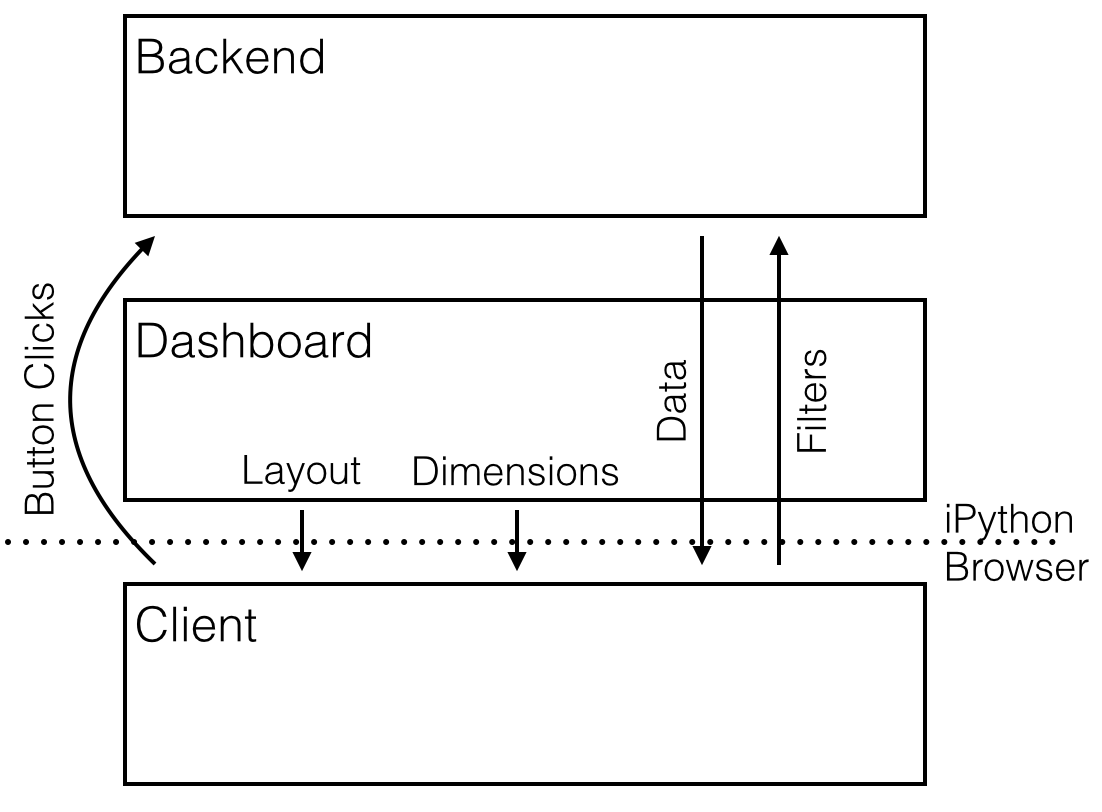
\includegraphics[width=3in]{figs/dataflow.png}
	\end{center}
	\caption{Data flow within the iDcDashboard system}\label{fig:system_flow}
\end{figure}

To ease implementation and extensibility we segmented the iDcDashboard system into three layers: the backend layer, the dashboard layer, and the client layer.
These three layers communicate as seen in figure \ref{fig:system_flow}.

The dashboard is the central layer and serves two main purposes.
First it exposes a simple python interface to configure the javascript based client layer.
Second it provides an interface for two way communication between the client and the backend.
This layer is the main layer a user will interact with.

The client layer renders the plots at the users request and orchestrates what data the plots display.
A plot interface allows easy addition of new plot types to the system without knowledge of the backend coding or the iPython widget complexities.

The backend is a facade class to provide a consistent interface between the dashboad and a dataset object.
The isolation from the direct widget allows easy addition of a backend supporting additional data sources or data processing procedures.

We now go into detail on each of these three layers individually.

\subsubsection{Dashboard}\label{sec:dashboard}

The dashboard class serves as the middleware between the backend and the client.
Upon construction, the object creates and configures the client and registers itself with the backend.
Once constructed it exposes two communication pipes which are used for two way communication between the backend and the client.
An ancillary function is that it renders the backend's toolbar to allow user calling of backend functions.

The constructor of the dashboard accepts three parameters: the backend object, a list of dimensions to create, and a list of rendering directives (plots and layout engine commands).
Details of the dimension and rendering directives themselves will be discussed in section \ref{sec:api}; however, they are effectively a DSL for the generation of the client's JSON configuration discussed in section \ref{sec:client}.
After configuring the client, the dashboard registers itself with the backend (thus telling the backend where to push new data to) and renders an optional toolbar provided by the backend (this toolbar provides a direct interface to the backend).
Once constructed, the main function of the dashboard is to provide two pipes between the backend and the client.

The data pipe is used by the backend to override the data in the client with a new set of data.  
The pipe uses a JSON blob containing a single JList of JObjects.
Since the system is only designed to handle tabular datasets, the JObjects are expected to be flat, that is only contain strings or numerics for values.
To ease backend programming the dashboard also accpets Pandas DataFrame or Python lists of dictionaries which it will automatically convert to the correct JSON blob format.

The filter pipe is used by the client to inform the backend of any filters applied on the client side.
Two kinds of filters are supported: set inclusion and numeric range filters.
A set inclusion filter is a single JArray containing the values the analyst has selected.
Range filters are stored as a JArray of JArrays specifying min, max pairs of the ranges selected in the client.
When multiple filters are applied to the same field, the union of the sets accepted by each filter is accepted.
The dashboard provides some preprocessing of the dashboard to ease interpretation by the backed, primarily converting filters from being over dimensions to being over fields in the raw data.

\subsubsection{Client}\label{sec:client}

The client is a collection of JavaScript objects which work together to render the desired plots.
The key components are the layout engine,  the plotting code, and the data manager.

The layout engine interprets a layout configuration provided in JSON format.
The JSON configuration is a JArray of JObjects describing objects to render.
All objects to be rendered have a type field which specifies which object to render.
There are two distinct classes of objects which can be rendered, layers and plots.
A layer creates a new div as wide as the rendering area which has a specified height.
All plots will be rendered into the last defined layer.
An example of this semantic is displayed in figure \ref{fig:layout}, note how the first two plots (the bar and scatter) render within the first row and the third plot renders in the second row.
A plot object contains configuration describing the plot, typically the data source it will plot from, the width, and plot type specific configuration directives.
The layout engine creates a div within the previous layer's div and passes it as a target for the plotting code to render the defined plot onto.

\begin{figure}
\begin{lstlisting}
[{type:layer, height: 300}, 
  {type:bar,  ...},
  {type:scatter, ....},
  {type:layer, height 200},
  {type:row, ...}
]
\end{lstlisting}

\begin{lstlisting}
[
  Layer(300), 
  Plot("bar")..., 
  Plot("scatter")...,
  Layer(200), 
  Plot("row")
]
\end{lstlisting}
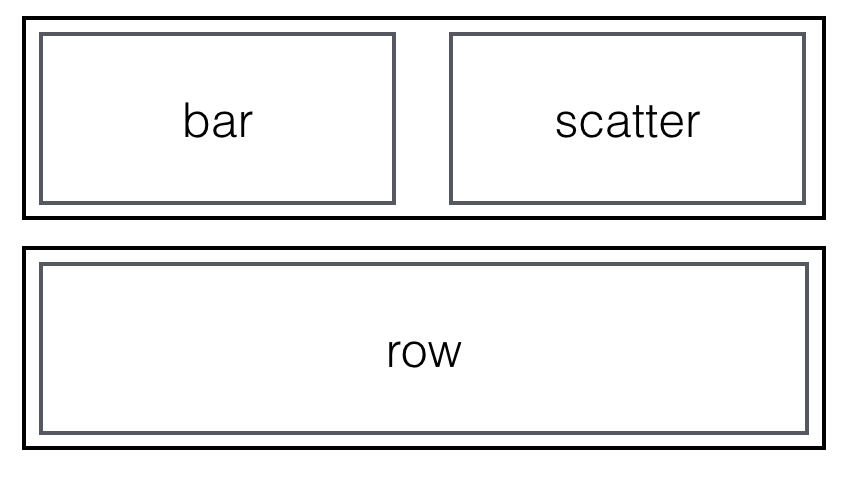
\includegraphics[width=3in]{figs/layout_example.png}
\caption{\emph{(Top)} Example configuration code for client layout engine along with \emph{(Middle)} the Python code to generate said configuration.  Finally \emph{(Bottom)} a diagram showing how the plots will be rendered.}\label{fig:layout}
\end{figure}

While the layout engine creates the divs for laying out plots, the actual plotting is done by specialized classes for each plot type.
The type field of the configuration object is used to look up the specific object get.
All plot objects define a render, set\_data\_source, update\_data, height, and width methods which are used to control the creation of the object.
In addition to the standard object creation methods, an additional set of plot specific configuration methods can be defined.
We have used this to implement setting of domain and range on x/y coordinate plots, setting axis labels, and other useful options.
In the current system, all plottable objects come from the dc.js package but this interface in general enough that we belive other plotting libraries or even raw HTML generation code could go in this framework.

Finally, the data manager of the client holds the data passed from the server and connects plots to the data they are configured to plot.
To hold the data, Square's Crossfilter.js\cite{crossfilter} library is used.
Crossfilter provides an data structure which holds JSON records and allows for quick and efficient sorting and selection to support the interactive plots.
To support this, Crossfilter creates \emph{dimension} and \emph{group} objects on the data.
A dimension converts the arbitrary records into a plottable series of either a single data point per row or a (x,y) pair of points per row.
A group defines a map-reduce function which collects points in a dimension together and then replaces the grouped points with a single value.
A typical use of a group is to create a binned histogram of a dimension by mapping the dimension to a bin and then reducing by counting the number of records in each bin.

The data manager accepts a JSON configuration for creating dimensions/groups and assigning each dimension and group a name.  
This is done by passing a JObject where keys are dimension names and values are annother JObject describing the given dimension.
A dimension's JObject contains the javascript code for mapping a record to the points and an object describing all the groups in a similar manner as the dimensions.
The data manager then allows referring to a dimension and group by the name ``cf/(dim name)/(group name)'' and by default creates a null group which uses an identity mapping for points and returns the count for each distinct value.

\subsubsection{Backend}\label{sec:backend}

The backend's job is to provide data to visualize.
Typically the backend is simply a facade over a standard data set providing object or a network connection to a remote dataset.  
However, it is possible to create a backend that produces data or performs more complicated data processing tasks.

There are two ways for the user to interact with the backend.
First the backend exposes a toolbar which is a collection of standard iPythonNotebook widgets (typically buttons and other standard form items) which have call back functions into the backend.
This allows the backend to have specialized user interaction such as allowing the user to request a new dataset be pushed.
Secondly, every time a filter is modified on a plot the client notifies the backend as described in section \ref{sec:dashboard}.
Each time either of these events happen the backend can decide to push a new dataset to the dashboard/client as described in \ref{sec:dashboard}.

A very simple backend is the standard Backend.DF\_Backend which accepts a Pandas DataFrame and pushes it to the dashboard upon dashboard registration.
This backend never pushes a new data set and is suitable for analysis of small static datasets.
A set of more powerful backends capable of plotting bigger or dynamic datasets is described in section \ref{sec:bigdata}.
It is expected that most extension/customization of the iDcDashboard system will come in the form of new backends to handle different kinds of data sets.

While the big data dashboard described later simply use filters to resample data, the backend is able to do any arbitrary action.  Some discussed ideas which are left to future work are:
\begin{itemize}
	\item Interactive training of models on subsets of data
	\item Modifying the backing data store by adding a value to records selected by filter
	\item Plotting of streaming data as it is coming in
	\item Using multiple backends and dashboards together to see different aspects of the data
\end{itemize}
We suspect the iDcDashboard system to stand up to all of these potential uses.

\subsection{Programming Interface}\label{sec:api}

To use iDcDashboard, the user creates a new instance of the Dashboard object by passing three parameters: the backend, list of dimensions, and layout configuration.

As described in section \ref{sec:backend}, the backend is a python object which connects to a data source the user wishes to analyze.
The data is provided in a single json list containing flat json objects of key/value pairs.

Dimensions are configured via the Dimension and Group classes which provide automatic generation of the data manager configuration discussed in section \ref{sec:client}.
An example of the dimension configuration is seen in \ref{fig:simple_example}.
A dimension is either a single column (used for the primary axis on most plots) or a pair of columns (used for (x,y) scatter plots) from the dataset.
A group describes how to compute the secondary axis on single column dimensions.
The majority of plots use a single column dimension and group to specify a function from dimension value $\mapsto$ group value,
however, a scatter plot uses a pair dimension to show a collection of points in a scatter plot design.
All dimensions and groups are assigned a name to identify it in plot creation.
By default a single column dimension is named ``field\_name''  and a pair dimension is named ``field\_1\_field\_2'' however the name\_override parameter can be passed to a dimension to give a custom name.
All groups must be manually named.

The configuration of plots is done by passing a list of Layer and Plot objects. 
This provides an abstraction over the layout engine JSON configuration described in section \ref{sec:client}.
The layer constructor accepts a single parameter describing the layer height.
The plot constructor accepts the type of the plot (bar, scatter, and pie are example types) and then uses the builder design pattern of having configuration methods to apply further configuration.
The most important method is the data\_source method, which accepts two parameters, the dimension and group (defaults to an neutral group).
Additional methods (title, width, etc) control the formatting of the plot.
In order to support plot specific configuration settings, the method ``config'' is used.
The config method accepts a variable name followed by a list of parameters.
Config is used for plot specific things (domain/range of a scatter, color of points, etc) and must be documented for each plot.

\begin{figure*}[hb]
\begin{lstlisting}
Dashboard(
  Backend.DF_Backend(data_frame), 
  [
    Dimension("field_1","field_2"),
    Dimension("field_3", name_override = "third field").
      add_group("rounded",Group("function(d){return 20*Math.floor(d/20);}"))
  ],
  [
    Layer(200),
    Plot("scatter").data_source("field_1_field_2").width(400),
    Plot("bar").data_source("third field","rounded").width(400)
  ]
).show()
\end{lstlisting}

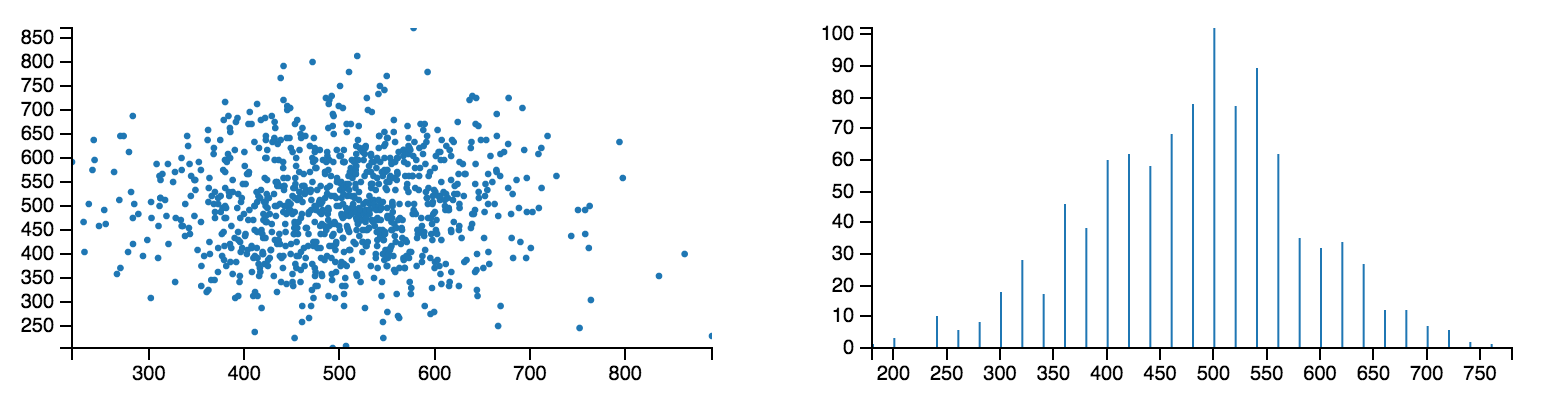
\includegraphics[scale=.63]{figs/screenshot_scatter_bar.png}
  \caption{\emph{Above:} basic code to create a scatter plot and bar plot of a Pandas data frame.  \emph{Below:} the resulting plots.}\label{fig:simple_example}
\end{figure*}

\section{Scaling to Big Data}\label{sec:bigdata}%2 pages
Scaling to large data is handled in two stages.  In the first stage we assume the data is small enough to fit in the memory of the iPython run time.  We then scale the solution for this up by using an Apache Spark cluster as a data store which we access through a restful api.  We discuss these two solutions separately.

\subsection{iPython Resident Datasetets}
In the first stage, the dataset is small enough to fit within iPython's memory and thus the two bottlenecks are sending data from python to the client widget and memory constraints on the client side.
In experiments, dc.js had difficulty handling more than 10,000 records before experiencing lag in the UI.
Furthermore, given a typical plot in a dashboard would be ~400x400 or 160,000 total pixles 10,000 points will often saturate most of the anticipated plots.  
Finally, since each record will usually be several hundred bytes 10,000 records will be a few megabytes which we suspect to be sufficiently small to transfer to the client without much delay on a modern internet connection.
Thus we decide that we only need to display 10,000 simultaneous data points on any data set.

To visualize data sets that fit in iPython's memory, we store the data in a pandas data frame.
To keep the displayed data size down, we simply sample the records of the data frame and then send them down to the client.
We allow the user user to resample at any time by exposing a UI button which triggers the data refresh.
When the data is resampled we select the sample the records from only the data that matches the currently applied filters.

This allows the following work flow:
\begin{itemize}
	\item User is displayed a random sample of the whole data set
	\item User highlights data they are particularly interested in
	\item User clicks resample
	\item User now has a zoomed in view of just the data they are interseted in and can futher explore just that region.
\end{itemize}

In addition, we expose additional UI buttons which allow marking of all data matching the currently applied filter.
This allows the user to label data for supervised learning, select data for further statistical analysis, or any other thing which may be interesting.

\subsection{Remote Datasets}\label{sec:big_data_remote}

While the first stage of scaling solves the scaling issue to data sets which are loadable in python, it limits the scale to things that can fit in pandas on a single server.
Larger data sets or streams of data (IE twitter data) cannot fit into this model since they cannot fit into a single servers memory and often are changing in nature and thus cannot be put into a static pandas data frame.
This problem is solvable by creating custom backend objects for the users specific needs.
In this section we describe the HTTPS Backend coupled with the Restful RDD project which allows arbitrarily large data sets to be visualized in an interactive manner.
The target work flow is the same as in the first stage.

Data is stored within a Apache Spark RDD containing record objects.  A webservice was written in Scala using the Scalatra web framework which connects to the Spark instance containing the RDD and exposes a restful API for acquiring samples of the data suitable for pushing to the front end.  Again we sample the data to be on the order of 10,000 records so the front end can have no slowness so we suspect the data will be small enough that the HTTP transfer of the data will be minuscule.

The REST API used in this system has the following interface.
A POST request is made containing the parameters of the dataset the iDcDashboard requests.
The parameters of the request include the number of records to be sampled, the sampling method, and a list of filters to apply to the data.
The body of the response gives a dataset id.
The iDcDashboard then makes a GET request with the dataset id every second until the data is ready.
The dataset is in the form of a JArray of JObjects for each record.
Once the data is downloaded, it is pushed to the client.

\section{Performance Evaluation}%1 page

To evaluate performance, we believe the time to re-sample a large data set and the time to plot the data set are the most critical.
To do this we perform tests on two data sets/dashboards.

\subsection{Local Backend}

Our first experiment tests our local sampling backend.
We use a cut of NOAA US historical weather data containing 4.2 million temperature measurements which stores to a 300 MB file.
We designed a dashboard containing eight distinct plots: a scatter plot of measurement latitude/longitude, a pie chart of measurements state, a scatter plot of temperature/day of year,  a histogram of temperature, a histogram of day of year binned into 5 day chunks, a histogram of year binned to nearest decade, and a pie chart of quarter of year.
A screenshot of this dashboard can be seen in the appendix.

To evaluate performance we measure the time between clicking the resample button until the data has completed pushing to the client and the time from the client receiving the data until the plots have finished rerendering.
We perform this test with exponentially increasing sample sizes of 100, 1000, 10000, 100000 data points 5 times per sample size.
At the sample size of 100 and 1000 the tools were all very responsive; however, at 10,000 it took a few seconds for the scatter plot to respond however the other plots took under a second and still felt reasonable.  
At 100,000 data points the gui was extremely difficult to use and could be considered unuseable.

\begin{figure}
\begin{center}
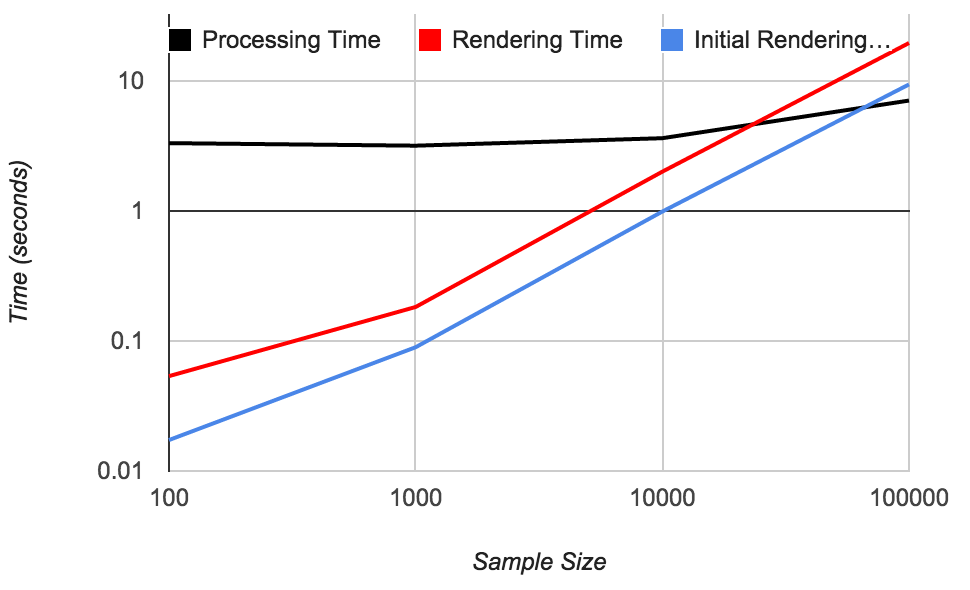
\includegraphics[width=3in]{figs/weather_perf.png}
\end{center}
\caption{Average processing and rendering time for local sampling data set.  Both axes are on a log scale}\label{fig:weather_perf}
\end{figure}

The results of this experiment are presented in figure \ref{fig:weather_perf}.
We see that processing time is nearly constant and only increases signifantly at a sample size of 100,000.
Additionally we see that the rendering time is approximately linear but typically faster than processing time until we hit 100,000 records.
An interesting discovery is that initial rendering time, the time it takes to render the plots using the initial sample, is consistently about half the time of the resampling rendering time.
It is likely that the data loading routine is called before the data has finished transfering to the client increasing the render time while the data is already there before the initial render.
These rendering times seem reasonably fast and within the range of time an analyst would be willing to wait for such a process, especially given the alternative of manually filtering/processing and then plotting would take more time and require more effort.

\subsection{Remote Backend}

After evaluating the performance of a local data provider we turn our attention to evaluating the performance of a remote back powered by Apache Spark and a REST API described in section \ref{sec:big_data_remote}.  
We do two performance evaluations, first of a larger sample of the weather data and then a new dataset/dashboard of twitter data.

We used a Spark cluster consisting of 15 nodes with 16 cores per node and 20 GB of ram per node.
The file was partitioned into 960 partitions (4 per core).
Prior to our experiments, a count of number of rows in the data set was performed and the data was cached.
This took about 1 minute of processing time but would only have to be done once assuming the cluster has sufficient memory to hold the dataset.

\subsubsection{Weather Data}

The larger weather dataset is similar to the local version; however, it contains weather from the whole world to get 300 million temperature measurements (about 100x larger than the local version).  
The data set was approximately 2 GB after processing.
We perform a similar experiment as before; however, this time we measure multiple elements of the processing time.
In particular, we measure the amount of time Spark spent processing the data and the total processing time as seen by iDcDashboard.
Additionally measurements of the time spent between downloading the data and pushing it to the client; however, this time was found to be trivial and too small to plot.

\begin{figure}
\begin{center}
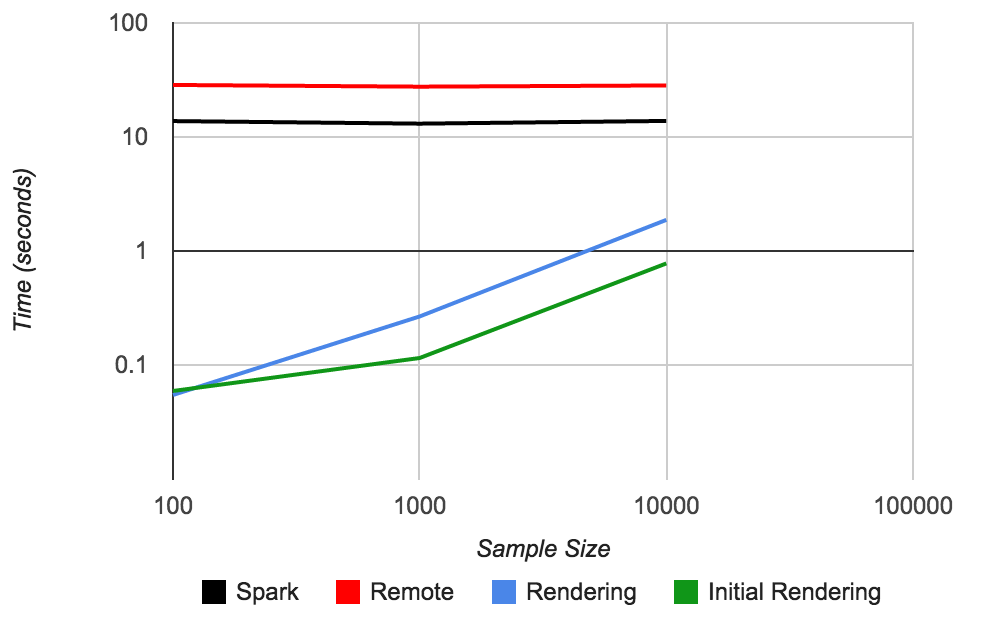
\includegraphics[width=3in]{figs/weather_big_perf.png}
\end{center}
\caption{Average processing and rendering time for remote sampling weather data set.  Both axes are on a log scale}\label{fig:weather_big_perf}
\end{figure}

The results of this experiment are presented in figure \ref{fig:weather_big_perf}.
Sampling time and spark execution time are constant, which matches results on the local machine;
however, interestingly spark execution time accounts for only one half of the total sampling time.  
This is probably caused by network latency between the spark cluster to the web server and the websever to the iPython notebook.
Rendering times are inline with the local rendering time which is expected since the same dashboard was used and the backend has no impact on the rendering other than the data format (which is nearly the same).
Usability of the rendered dashboard was also the same as for the local case as expected.
We believe a 30 second round trip time to be reasonable performance given multiple layers of the system; however, it is likely many users will complain with this speed and thus demand a better solution.
Possible ideas are discussed in section \ref{sec:conclusion}.

\subsubsection{Twitter Data}

As a final experiment, we analyze a second data set consisting of data pulled using the twitter API.
This is still being worked out.

\section{Conclusion and Future Work}\label{sec:conclusion}%0.5 pages

In this paper we introduced the iDcDashboard, a novel system for exploratory visual analysis.


While the system's useability can be extended through additions of new plots and features, we believe the most significant work to be in improvements to the backend system.
Work to improve the remote backend's speed is particularly important.
A possible design would be to utilize a data hierarchy of client, ipython, webserver, spark with caching at each level to improve performance.
Due to the layered design it is expected this work will be easy to integrate into the system and is expected to take a couple of monhts.
Future work will also concern the use of this system to visualize data streams in an efficient manner and to identify areas this can be used for human guided machine learning.

This system was constructed over the Fall quarter of 2014 as David Lisuk's masters research project.
I would like to thank Professor Yoav Freund for advising me throughout this project, Julaiti Alafate for assisting with the administration of the Spark cluster and providing ideas, and my girlfriend Stephanie Lum for putting up with me through grad school.

\bibliography{bib}
\onecolumn

\section{Appendix}
\centering
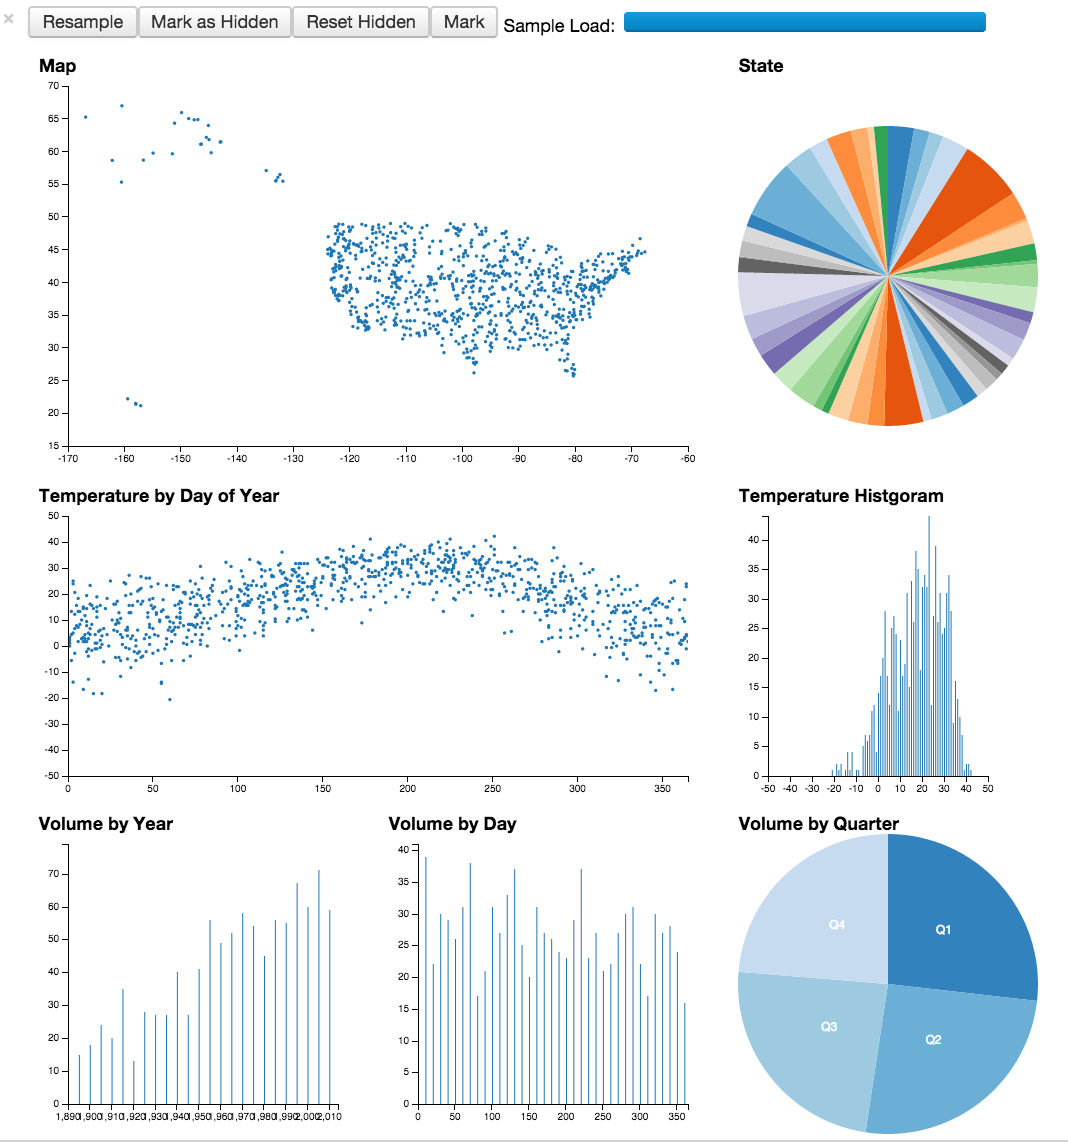
\includegraphics[width=6in]{figs/weather_dashboard.png}
\captionof{figure}{Screenshot of weather dashboard used in performance evaluations}\label{fig:weather}

\end{document}